\documentclass[11pt]{article}

\usepackage{amsmath}
\usepackage{amsfonts}
\usepackage[margin=0.25in]{geometry}
\usepackage{listings}
\usepackage{color}
\usepackage{lipsum}
\usepackage{graphicx}
\usepackage{array}
\usepackage{mathabx}
\usepackage{amssymb}
\usepackage{joe}
\usepackage{titlesec}
\usepackage{multicol}


\bibliographystyle{plain}


\definecolor{dkgreen}{rgb}{0,0.6,0}
\definecolor{gray}{rgb}{0.5,0.5,0.5}
\definecolor{mauve}{rgb}{0.58,0,0.82}

\lstset{frame=tb,
  language=c++,
  aboveskip=3mm,
  belowskip=3mm,
  showstringspaces=false,
  columns=flexible,
  basicstyle={\small\ttfamily},
  numbers=none,
  numberstyle=\tiny\color{gray},
  keywordstyle=\color{blue},
  commentstyle=\color{dkgreen},
  stringstyle=\color{mauve},
  breaklines=true,
  breakatwhitespace=true,
  tabsize=3
}

\def\acts{\mathrel{\reflectbox{$\righttoleftarrow$}}}


\begin{document}


\section{Introduction}

We classify the free homotopy classes of loops on a once-punctured torus $T$ whose self-intersection number is four. In doing so, we present an algorithm for performing this classification for higher self-intersection numbers. Our method extends the work done by Butler, Carton, and Kraft in \cite{geo3} and Crisp et al, in \cite{geo2}.\\

Our classification considers the action of the mapping class group. So, we identify two free homotopy classes if there is a self homeomorphism of $T$ taking one class to the other. By the Dehn-Nielsen-Baer Theorem, this is equivalent to classifying free homotopy classes up to automorphisms of the fundamental group $\pi_1(T)$. Since $\pi_1(T)\cong F(a,b)$, the free group on two letters, it suffices to consider the automorphisms generated by the following elementary transformations.
\begin{equation*}
\alpha=\begin{cases} a\mapsto b\\ b\mapsto a\end{cases},
\beta=\begin{cases} a\mapsto ab\\ b\mapsto b\end{cases},
\gamma=\begin{cases} a\mapsto a^{-1}\\ b\mapsto b\end{cases}
\end{equation*}
In particular, these transformations, and hence all automorphisms of $F(a,b)$, fix the boundary component (the puncture) $aba^{-1}b^{-1}$. The free homotopy classes themselves of $\pi_1(T)$ correspond to conjugacy classes of words in $F(a,b)$. For the sake of brevity, we will denote the letters $A$ and $B$ to mean $a^{-1}$ and $b^{-1}$, respectively, in the rest of this paper.\\

If we equip $T$ with a hyperbolic metric, we may also classify the geodesics of a given self-intersection number, up to homeomorphism. In fact, a geodesic has the minimal number of self-intersections amongst all curves in its free homotopy class. The classification also does not depend on the particular metric. For more, see \cite{geo2}.


\section{Simple Loops}

We view a loop as a continuous map from $S^1\to T$. A loop is said to have a nontrivial self-intersection if the loop has a single transverse intersection, and is not freely homotopic to a simple loop. A loop is said to have $k$ nontrivial self-intersections if it has $k$ transverse self-intersection points and if it is not freely homotopic to a loop with less nontrivial self-intersections or to a simple loop. A free homotopy class is said to have intersection number $k$ if it contains a loop with $k$ nontrivial self-intersections. It should be clear that this is well-defined since we only consider non-trivial intersections.\\

We start by classifying simple loops using the same lemmas and theorems from \cite{geo3} and \cite{geo2}. We provide different proofs of some results from \cite{geo3}. Using these, we can write any loop with four self-intersections as a composition of five simple loops.

\begin{thm}
The automorphic conjugacy class (or orbit) of a simple loop $\ell$ on $T$ is either
\begin{itemize}
\item the identity, and $\ell$ bounds a disc,
\item one of $[abAB]$ or $[baBA]$, and $\ell$ bounds a punctured disc
\item $[w]$ where $w$ is a generator of $\pi_1(T)$, and $\ell$ does not separate $T$
\end{itemize}
\end{thm}
\begin{proof}
See \cite{geo1}
\end{proof}

\begin{thm}
Up to free homotopy any $\ell$ on $T$ with $k$ transverse self intersections points can be formed as the composition of $k+1$ simple loops which intersect at a single point.
\end{thm}
\begin{proof}
See \cite{geo2}
\end{proof}

The simple loop decomposition of a curve with $k$ self-intersections must, in fact, only contain nontrivial simple loops. For, if a simple loop exists in the decomposition, then it either arises from a simple loop in the original curve (which is impossible since our intersections are nontrivial) or a bygone shown below in the original curve
\begin{center}
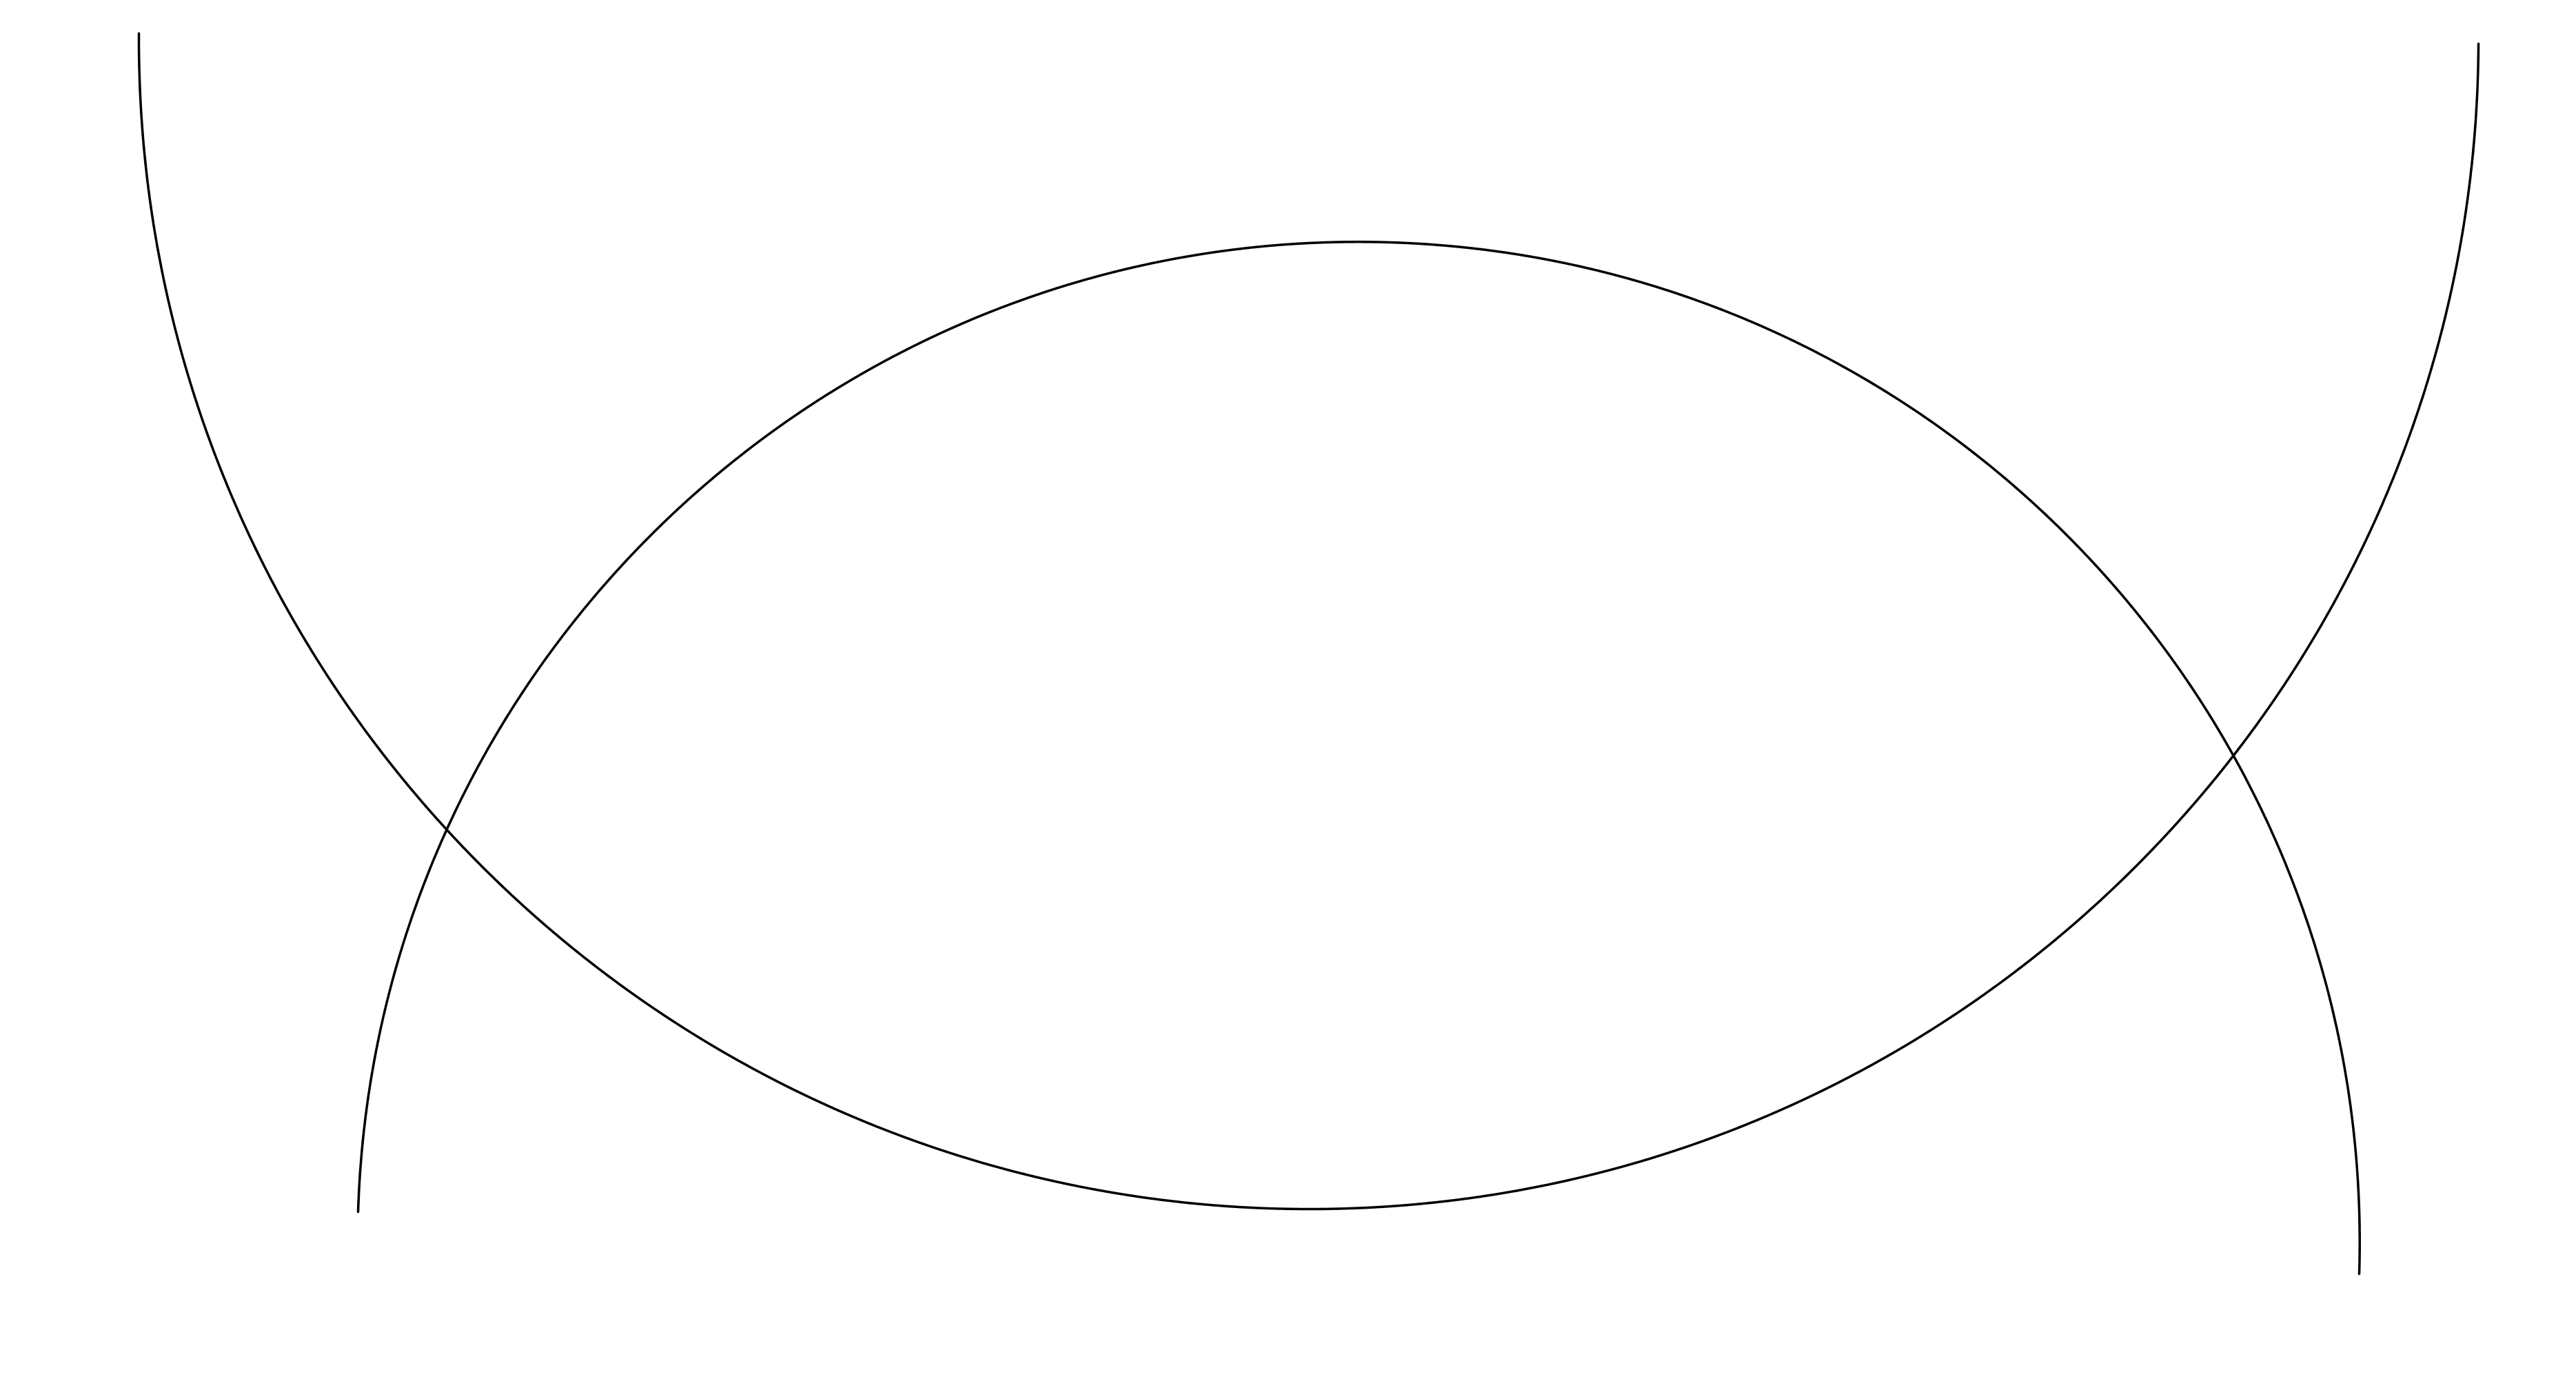
\includegraphics[scale=0.05]{bygone.png}
\end{center}
Here, the simple loop is formed when the segment of the curve with the two distinct intersection points as endpoints is "collapsed". For more, see the proof of Theorem 2.2 in \cite{geo2}. In either case, we have trivial intersection points.

\begin{thm}
Let $\{a,b\}$ be a generating pair for $\pi_1(T)$. Let them intersect at a basepoint $x$. Then, any other element in the automorphic conjugacy class of a generator of $\pi_1(T)$ which only intersects $a,b$ at $x$ is representable by one of the following, up to orientation and reflection.
\begin{itemize}
\item $a$
\item $b$
\item $baB$
\item $abA$
\item $ab$
\end{itemize}
\end{thm}

\begin{proof}
We cut along $a$ and $b$ to get a translation of the fundamental polygon for $T$. The vertices of the polygon are identified as the basepoint $x$, whereas the cross represents the puncture of the torus. We choose an orientation and draw simple loops from the bottom-left basepoint. Up to homotopy, it's clear the possibilities are given by the following
\begin{center}
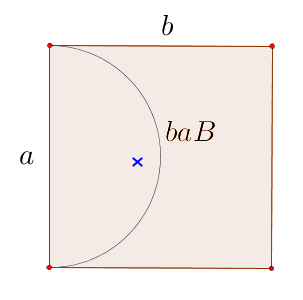
\includegraphics[scale=0.5]{baB.png}
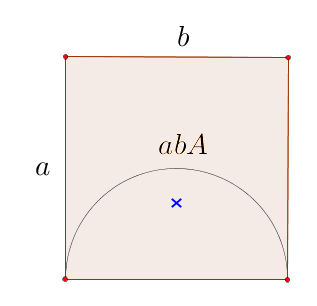
\includegraphics[scale=0.5]{abA.png}
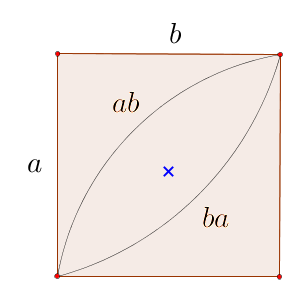
\includegraphics[scale=0.5]{ab.png}
\end{center}
Otherwise, it is clear that our loop will be homotopic to either $a$ or $b$.
\end{proof}

We observe that all outer automorphisms of $T$ fix the puncture $abAB$ since the generators do. Thus, our simple loop decomposition of a given curve with $k$ self-intersections must consist of only those listed above or the loop bounding the puncture $abAB$.

\begin{thm}
Let $\{\ell_1,\ell_2,\ldots,\ell_n\}$ be a collection of non-homotopic simple loops in the orbit of a generator of $\pi_1(T)$ which intersect only at a basepoint. Then $n\leq 4$ and generators for $\pi_1(T)$ can be chosen so that $\{\ell_1,\ell_2,\ldots,\ell_n\}$ is one of
\begin{itemize}
\item $a$
\item $a,b$
\item $a,baB$
\item $a,b,baB$
\item $a,b,ab$
\item $a,b,ab,abA$
\end{itemize}
\end{thm}
\begin{proof}
Since all our $\ell_i$ are in the orbit of $a$, WLOG, we can always assume one of them is $a$ and select the other simple loops accordingly. We divide our work into cases depending on whether there is a loop homotopic to $b$ in our arrangement or not.\\

Suppose such a loop does exist. For $n=2$, we must have $\{a,b\}$ as our arrangement.\\

For $n=3$, we can have $\{a,b,ab\}$, $\{a,b,baB\}$, and $\{a,b,abA\}$ by Theorem 2.3. However, the fundamental polygons of $\{a,b,baB\}$ and $\{a,b,abA\}$ are equivalent up to rotation. Thus, there is a homeomorphism of $T$ taking one to the other.\\

For $n=4$, we can have $\{a,b,abA,ab\}$ or $\{a,b,baB,ba\}$ which also give the same fundamental polygons up to rotation and reflection. $n>4$ is not possible due to Theorem 2.3.\\

Suppose a loop homotopic to $b$ is not in our arrangement. For $n=2$, we can have $\{a,baB\}$. Next, we have two sub-cases determined by whether our arrangement contains loops crossing $b$ in the fundamental polygon or not. If such crossing loops do not exist, then we are restricted to the loops given by Theorem 2.3. We have both $\{a,abA\}$ and $\{a,ab\}$ (and hence $\{a,ba\}$) are automorphic to $\{a,b\}$ as seen by the following diagrams
\begin{center}
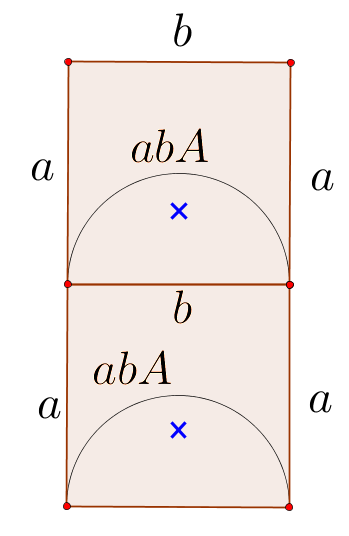
\includegraphics[scale=0.5]{aabA.png}
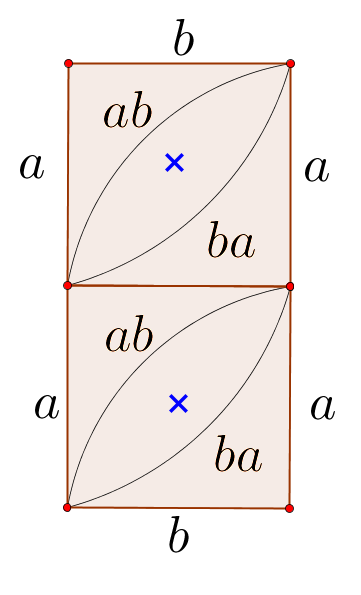
\includegraphics[scale=0.5]{aab.png}
\end{center}
which are translations and dilations of the fundamental polygon determined by $\{a,b\}$. Hence, any further arrangements in this sub-case for $n>2$ will merely be repeats of our cases for $n>2$ containing $a,b$ loops.\\

Now, suppose our arrangement contains loops crossing $b$ in the fundamental polygon. With a fixed orientation, we can draw loops emanating from the bottom left identified basepoint. It can return to a basepoint either on the left side of the fundamental polygon or the right side, shown respectively below
\begin{center}
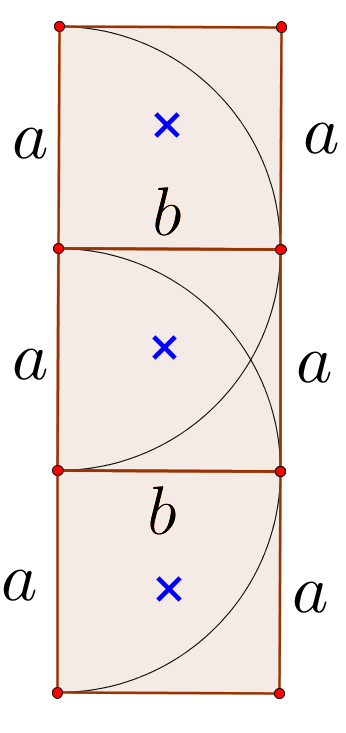
\includegraphics[scale=0.5]{crossb1.png}
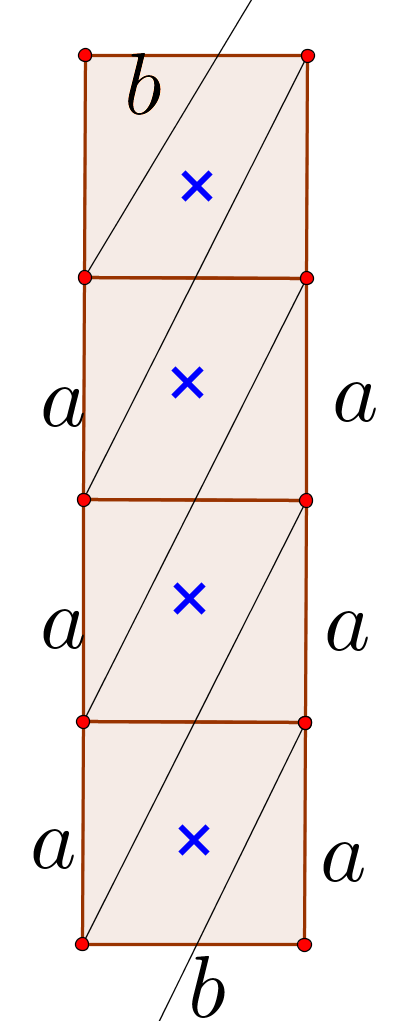
\includegraphics[scale=0.5]{crossb2.png}
\end{center}
WLOG, for the first case, our arrangement is clearly impossible since the curve must cross itself if it crosses $b$ and returns to a basepoint on the left side again (contradicting our loops being simple). For the second case, we again arrive at a dilation and rotation of the $\{a,b\}$ fundamental polygon. Thus, further arrangements for $n>2$ will be automorphic to one of our $a,b$ arrangements for $n>2$ from before.
\end{proof}

\begin{cor}
Any configuration of five non-trivial simple loops on $T$ is automorphic to one of a finitely many given lists of words.
\end{cor}


\begin{proof}
If the simple loops are pairwise non-homotopic, then this is simply Theorem 4. Otherwise, consider the arrangements given by Theorem 4 with duplicates of words.
\end{proof}

\section{Basepoint Diagrams}


\subsection*{Basepoint Graph}

Given a closed curve $\gamma$ on our surface $S_{g,b}$ with $k$ self-intersection points, use Lemma 3 to obtain a curve with all of its intersection points contained in some small neighborhood $N_k$ (but not at the same point). Now, we would like to know two things:
\begin{enumerate}
\item How is the curve traversed outside of $N_k$?
\item How is the curve traversed inside of $N_k$?
\end{enumerate}
To answer (1), we may contract the neighborhood $N_k$ into a single point (using Lemma 3) so that our curve is now indeed a composition of $K+1$ simple loops. The nature of these simple loops (such as asking what are their complements, how many are homotopic to each other, etc.) is well-defined for a given curve $\gamma$.\\

To answer (2), if we imagine $N_k$ as an open disk with some boundary $\partial N_k$, then we know that $\partial N_k$ will contain $2(k+1)$ distinct points since the curve must enter each of the $k+1$ simple loops described in the answer to (1) and also exit each of them exactly once.\\

Each $\gamma$ induces an embedded graph $G$ on our surface $S_{g,b}$. Let the vertices of $G$ be the $k$ intersection points of $\gamma$. Call a \bld{segment} the image of $\gamma$ between two (possibly non-distinct) intersection points. Thus, the segments are the edges of $G$. We call $G$ the \bld{basepoint graph} induced by $\gamma$.\\

We observe that there is a total of $\frac{4k}{2}=2k$ segments (counted four times for each intersection point and overcounted by $2$). Each of the simple loops is also a single segment. Thus, there are $2k-(k+1)=k-1$ segments entirely contained within $N_k$ (for a fixed $\gamma$).\\

We have that $\gamma$ also induces a planar graph  $\bar{G}$ contained inside $N_k$. This is simply the maximal subgraph of $G$ contained inside $N_k$. In other words, we eliminate all edges of $G$ which correspond to segments which are simply loops to obtain the subgraph $\bar{G}$. Here, the vertices still consist of the $k$ self-intersection points and the edges are segments between the $k$ intersection points contained inside $N_k$. Thus, there are $k-1$ edges now. We call this the \bld{reduced basepoint graph} induced by $\gamma$. We provide an example below by providing an image of a particular $\gamma$ inside $N_k$ and its induced basepoint graph and reduced basepoint graph.
\begin{center}
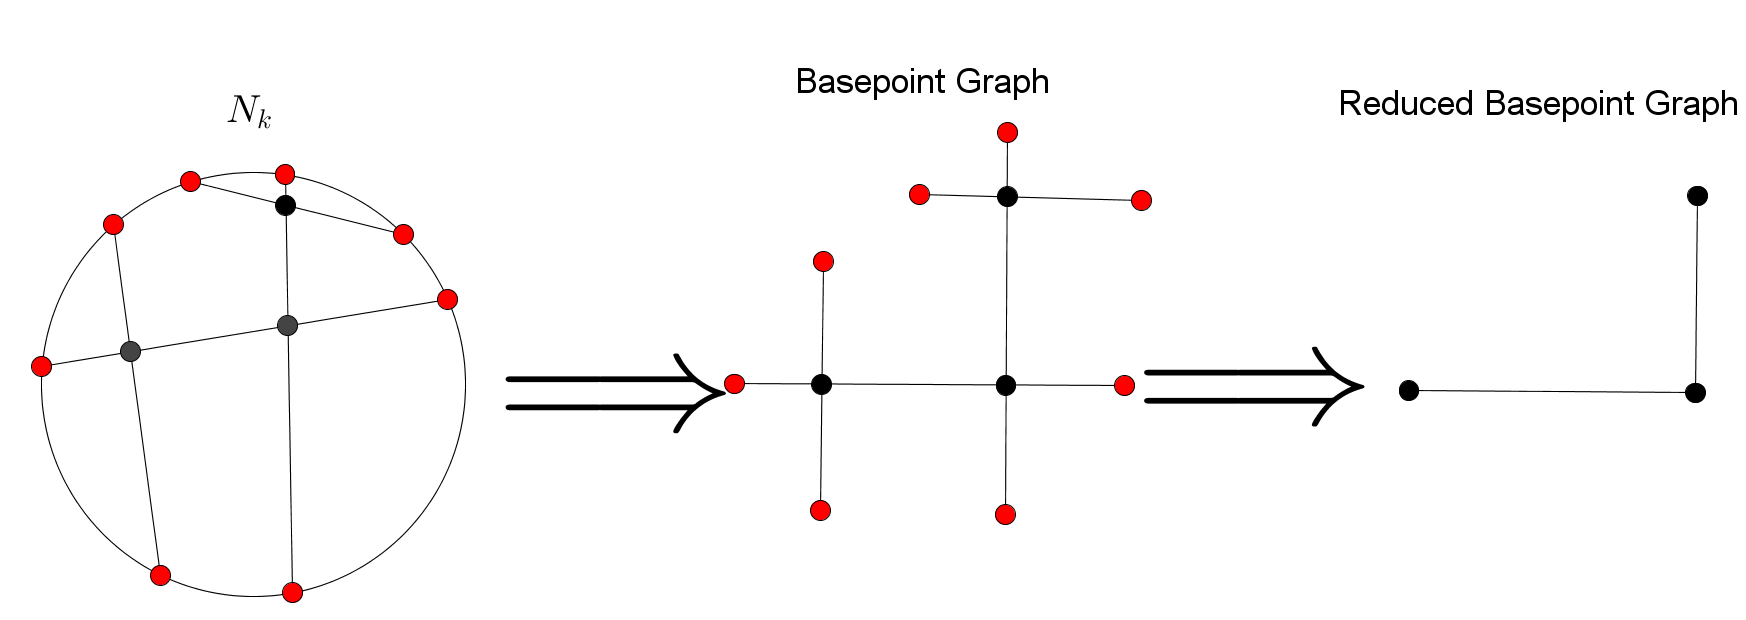
\includegraphics[scale=0.25]{basepointgraphconstruction.png}
NOTE: The red dots are not actual vertices of the basepoint graph, but merely act as placeholders for the simple loops (which connect two red dots)
\end{center}

\begin{remark} For a given $k$ and $\gamma$, it should be clear that there is only one basepoint graph associated to it. However, if we fix $k$ and let $\gamma$ range over all curves with $k$ minimal self-intersections, then there can clearly be many basepoint graphs associated to that $k$. Also, our choice of the neighborhood $N_k$ should not affect the basepoint graph either. Thus, the basepoint graph induced by a particular $\gamma$ is well-defined. In fact, it is well defined for $\text{Orb}([\gamma])$, the mapping class group orbit of the free homotopy class of $\gamma$, $[\gamma]$. Clearly, the action of free homotopy or self-homeomorphisms of the surface on $\gamma$ induce actions of graph isomoprhisms on the $G$ induced by $\gamma$.
\end{remark}

\begin{remark}
Ultimately, we would like to proceed backwards by enumerating all possible arrangements of $k+1$ simple loops intersecting at a single point (to understand all the possible ways $\gamma$ can behave outside of $N_k$)  and all possible reduced basepoint graphs (to understand all the possible ways $\gamma$ can behave inside of $N_k$). Then, we would have an exhaustive method of enumerating all the possible basepoint graphs of curves $\gamma$ embedded on $S_{g,b}$ with $k$ self-intersections. For each basepoint graph, we can easily find the complement of $\gamma$ with respect to the surface. The complement's components' topological types, equipped with the information of which intersection points lie on which components, completely determines an orbit. This is true since any free homotopy of $\gamma$, or the action of any self-homeomorphism of the surface on $\gamma$, induces a homeomorphism of the complement.
\end{remark}

\subsection*{Basepoint Diagrams for $k=4$}


\begin{prop}
For $k=4$, there are four reduced basepoint diagrams, shown below
\begin{center}
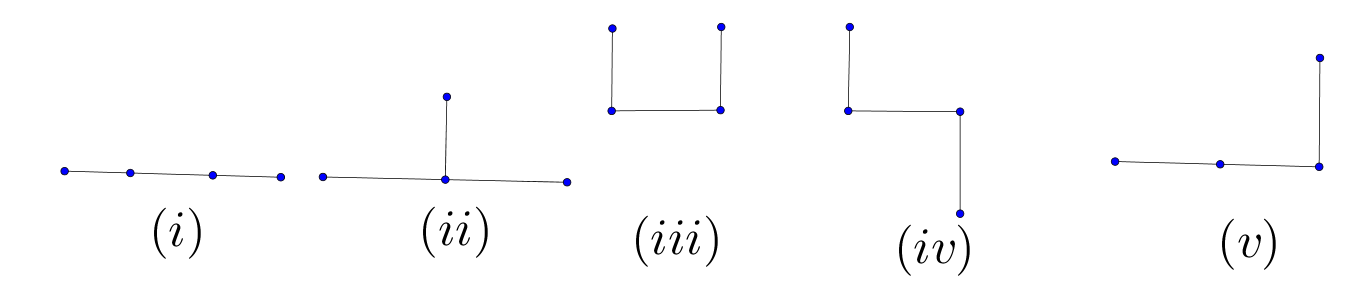
\includegraphics[scale=0.5]{basepointdiagrams4.png}
\end{center}
\end{prop}

\begin{prop}
Every closed curve with $k=4$ minimal self-intersections can be deformed into a composition of $5$ simple loops with basepoint diagram (v).

\begin{proof}
We suppose there is a curve that can be realized by basepoint diagram (i) (resp. (ii), (iii), (iv)) and not by (v) and show that it is (a) either a multicurve or (b) realizable by (v).\\

(TO BE FILLED IN).
\end{proof}
\end{prop}

\section{The Algorithm}

Given a particular simple loop arrangement and basepoint graph, we know exactly how the curve is traversed inside the basepoint neighborhood and the order in which the simple loops are composed. Thus, we know the word of the curve (i.e. its free homotopy class) in the fundamental group $F(a,b)$. Since the number of possible simple loop arrangements and the number of possible basepoint graphs are finite and given in the previous sections, we obtain an exhaustive list of free homotopy classes and, hence, of mapping class group orbits.

\begin{prop}
A free homotopy class of a closed curve on the punctured torus with four self-intersections is contained in one of the following $44$ orbits.
\begin{multicols}{3}
\begin{enumerate}
\item aaaaa
\item abaaBB
\item BabaaB
\item aabaaBa
\item aBBAbAB
\item aaBAABa
\item aBABABa
\item abaaBAB
\item abaaBaa
\item BabbbaB
\item abaBABa
\item BabbaBB
\item aBabaBB
\item aabAAAb
\item aabaBaa
\item abAbaaB
\item aaabAAAB
\item aabAABaa
\item aaabABaa
\item abbabABa
\item aBabABBAb
\item abAABAbaB
\item abABAbaBa
\item abaBAbABa
\item aBAbbaBAba
\item abbaBBabAB
\item aaabaBabAB
\item abbABabAAB
\item abaBAbaaBa
\item abAABBabAB
\item aabaBAbaBa
\item abbbaBAbaB
\item abaBABabab
\item aaabABabABa
\item aaabAABabAB
\item aabABabABaa
\item abABAbaBAbaB
\item abaBabABabABa
\item aabaBAbaBAbaB
\item abbaBabABabAB
\item aabABabABabABa
\item aabABabABabAAB
\item aabABabABabABabAB
\item abABabABabABabABabAB
\end{enumerate}
\end{multicols}
\end{prop}

\section{Distinctness}

\subsection*{Abelianization}

We observe that every closed curve (and its free homotopy class) on the punctured torus has a corresponding closed curve on normal torus. Two curves $\gamma_1,\gamma_2$ cannot be in the same orbit of our action if they are not on the same mapping class group orbit for the normal torus. This is equivalent to mandating that if two words in our list from the previous section are in separate automorphic conjugacy classes of $\mb{Z}^2$ after abelianization, then they must be in separate orbits of our action $MCG(T)\acts T$. Thus, to show distinctness of words (show that two words are indeed in separate orbits), it suffices to show distinctness of words in the same automorphic conjugacy class of $\mb{Z}^2$ after abelianization. We have the following result for four self-intersections.

\begin{prop}
The closed curve associated to each of the words found in Proposition 8 can be embedded on the normal torus and, if done so, belongs to one of the following automorphic conjugacy classes (orbits) of $\mb{Z}^2$:
\begin{multicols}{3}
\begin{itemize}
\item $[aaa]$ : \\
abaBabABabABa\\
aaabABabABa\\
aabaBAbaBAbaB\\
aabABabABaa

\item $[\text{Id}]$: \\
abABabABabABabABabAB\\
aaabAAAB\\
aabABabABabAAB\\
abABAbaBAbaB

\item $[aBa]$ : \\
abaBABa

\item $[A]$ : \\
abAABAbaB

\item $[B]$ : \\
aBabABBAb

\item $[BBB]$ : \\
aBABABa

\item $[baa]$ : \\
abAbaaB

\item $[aaaBB]$ : \\
aBabaBB

\item $[aaaB]$ : \\
abaaBB\\
BabaaB

\item $[baab]$ : \\
abbaBabABabAB

\item $[baba]$ : \\
abbabABa

\item $[bA]$ : \\
abbABabAAB

\item $[aa]$ : \\
abbaBBabAB\\
aabABabABabABa\\
aabAABaa

\item $[aBB]$ : \\
aaBAABa

\item $[a]$ : \\
aaabAABabAB\\
abaBAbABa\\
abABAbaBa\\
aabABabABabABabAB

\item $[AB]$ : \\
abAABBabAB

\item $[bAb]$ : \\
aabAAAb

\item $[aaB]$ : \\
BabbaBB\\
abaaBAB

\item $[BAB]$ : \\
aBBAbAB

\item $[abbba]$ : \\
BabbbaB

\item $[aaaaa]$ : \\
aabaaBa\\
aaaaa \\
aabaBaa \\
abaaBaa

\item $[aabab]$ : \\
abaBABabab

\item $[aaaa]$ : \\
aaabaBabAB\\
abaBAbaaBa\\
aaabABaa\\
aabaBAbaBa

\item $[bbaba]$ : \\
abbbaBAbaB

\item $[ba]$ : \\
aBAbbaBAba
\end{itemize}
\end{multicols}
\end{prop}

\subsection*{Whitehead's Algorithm}

We employ Whitehead's algorithm to prove distinctness of orbits in two steps.
\begin{enumerate}
\item For each word on our list (each candidate orbit), we find an element of minimal length in the orbit (if the element given in the list is not already minimal, we can arrive at a minimal word by applying elementary Whitehead transformations until we arrive at a minimal word).
\item Now, we have a list of minimal words. Two minimal words of different length clearly cannot be in the same orbit. Thus, it suffices to show distinctness for minimal words of the same length. However, the set of minimal words in a given orbit is finite and is, namely, the orbit of a given minimal word under the action of elementary Whitehead transformations. Thus, we can show distinctness algorithmically by finding each such orbit by iteratively applying these transformations to a single word on our list.
\end{enumerate}

\begin{prop}
We have the following characterization of our list where each each of the $44$ words found in Section 4 is followed by true if it is minimal in its orbit or else followed by a corresponding minimal word of its orbit.
\begin{multicols}{3}
\begin{enumerate}
\item abaBabABabABa : true
\item aBabABBAb : true
\item aBAbbaBAba : true
\item abbaBBabAB : true
\item abbbaBAbaB : true
\item aaabaBabAB : true
\item aaabABabABa : true
\item abbABabAAB : true
\item aaabAABabAB : true
\item BabbbaB : true
\item abaBABa : BBaaba
\item abaBAbaaBa : true
\item aabaaBa : true
\item abAABBabAB : true
\item BabbaBB : true
\item aabaBAbaBAbaB : true
\item abABabABabABabABabAB : true
\item abaaBB : true
\item aaabAAAB : true
\item aaabABaa : true
\item aBBAbAB : BAABaB
\item aBabaBB : bbaBaa
\item abAABAbaB : true
\item aaBAABa : true
\item abaBAbABa : true
\item aaaaa : true
\item aabAAAb : true
\item abABAbaBa : true
\item aabABabABabABabAB : true
\item abbabABa : true
\item abaBABabab : BABaaaa
\item aabaBAbaBa : true
\item aBABABa : BBaaaB
\item aabABabABabABa : true
\item aabaBaa : true
\item aabABabABabAAB : true
\item abaaBAB : aBBaba
\item abAbaaB : bbaaBa
\item abaaBaa : true
\item aabABabABaa : true
\item abABAbaBAbaB : true
\item BabaaB : true
\item aabAABaa : true
\item abbaBabABabAB : true
\end{enumerate}
\end{multicols}
\end{prop}


\begin{thebibliography}{9}

\bibitem{geo3}
Butler M, Carton J, Kraft E (1995)
Geodesics with Three Intersections on the Punctured Torus.
Proceedings of the REU Program in Mathematics, Oregon
State University.

\bibitem{geo2}
D. Crisp, S. Dziadosz, D. Garity, T. Insel, T. Schmidt, and P. Wiles (1998)
Closed Curves and Geodesics with Two Self-Intersections on the Punctured Torus.
REU Project follow-up paper, Oregon State University.
Mh. Math. 125, 189-209.

\bibitem{geo1}
Birman J, Series C (1984)
An Algorithm for Simple Curves on Surfaces.
J London Math Soc (2) 29:331-342

\end{thebibliography}



\end{document}
